\section{Littérature}
%\nocite{*}

%\begin{frame}[allowframebreaks]{Études de cas}
%	\printbibliography[keyword=case]{}
%\end{frame}
%
%\begin{frame}[allowframebreaks]{Études physiologiques}
%	\printbibliography[keyword=physiology]{}
%\end{frame}

\begin{frame}{Takekawa et al. (2021)}
	\centering
	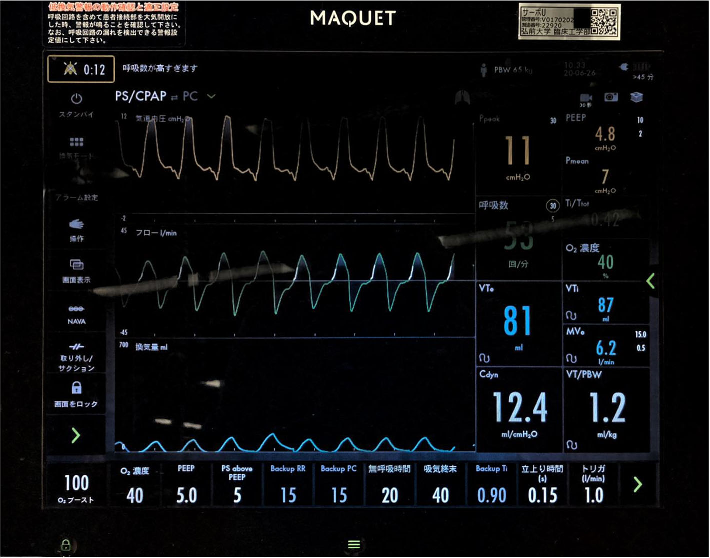
\includegraphics[clip, trim=20 5 22 25]{captures/Takekawa2021-1}
\end{frame}

\begin{frame}{Takekawa et al. (2021)}
	\centering
	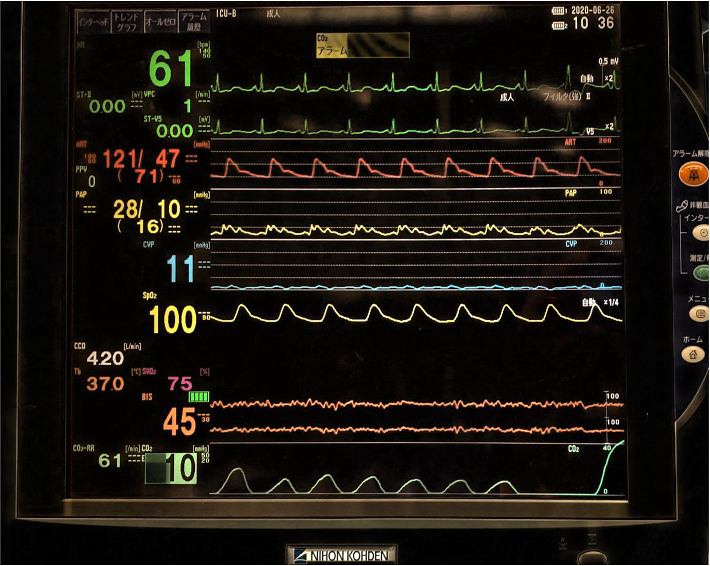
\includegraphics[clip, trim=33 0 35 15]{captures/Takekawa2021-2}
\end{frame}

\begin{frame}{Takekawa et al. (2021)}
	\centering
	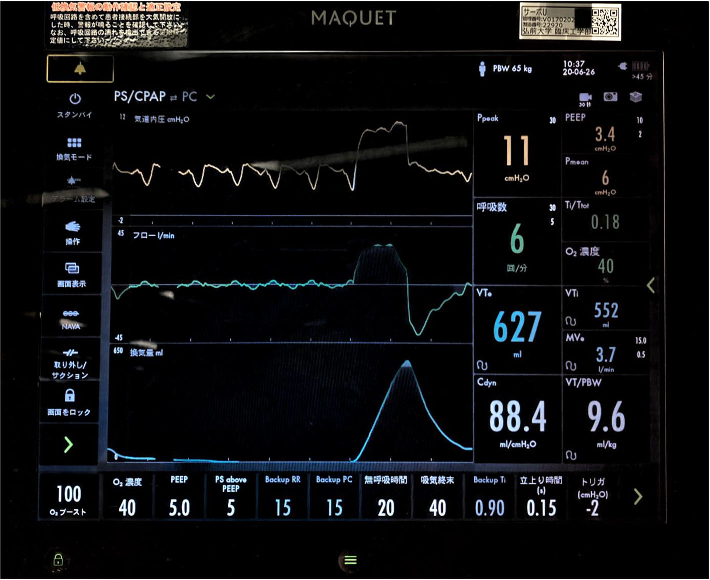
\includegraphics[clip, trim=20 5 22 25]{captures/Takekawa2021-3}
\end{frame}

\begin{frame}{Caractéristiques des autodéclencheur}
	\centering
	\def\mytblcolor{grischum}
	\rowcolors{3}{\mytblcolor!25}{white}

	\def\pa{p < .01}
	\def\pb{p < .05}
	\def\urvasc{dyne$\cdot$s/cm\textsuperscript{5}}
	\begin{tabular}{l >{\scriptsize}l c c >{\scriptsize}c}
		\hline
		\rowcolor{\mytblcolor!70}
		                              &          & FP   & Non-FP & \\
		\rowcolor{\mytblcolor!70}
		                              &          & n=23 & n=81   & \\
		\hline
		Résistances voies respi.      & \cmh/l/s & 8.5  & 10     & \pa \\
		Constante de temps            & s        & .41  & .49    & \pa \\
		Ratio cardiothoracique        & \%       & 61   & 58     & \pb \\
		Débit cardiaque               & l/min    & 5.5  & 4.2    & \pa \\
		Index cardiaque               & l/min/m² & 3,38 & 2,62   & \pa \\
		Volume d'éjection             & ml       & 60   & 48     & \pa \\
		Pression veineuse centrale    & mmHg     & 9,2  & 7,2    & \pa \\
		Pres. cap. plum . bloq.       & mmHg     & 10.9 & 8.7    & \pb \\
		Résist. vasc. systémique      & \urvasc  & 1278 & 1608   & \pa \\
		Résist. vasc. pulmonaire      & \urvasc  & 151  & 206    & \pa \\
		\hline
	\end{tabular}

	\adaptcite{imanaka_autotriggering_2000}
\end{frame}

\begin{frame}{Caractéristiques des autodéclencheur}
	\centering
	\def\mytblcolor{bleuclairchum}
	%\rowcolors{3}{marinechum!55!black}{normal text.bg}

	\def\pa{p < .01}
	\def\pb{p < .05}
	\def\urvasc{dyne$\cdot$s/cm\textsuperscript{5}}
	\begin{tabular}{l >{\scriptsize}l c c >{\scriptsize}c}
		%\hline
		%\rowcolor{marinechum!80!black}
		                              &          & Autodécl.   &
		Non-autodécl. & \\
		%\rowcolor{marinechum!80!black}
		                              &          & n=23 & n=81   & \\
		\hline
		\rowcolor{marinechum!80!black}
		Résistances voies respi.      & mbar/l/s & 8.5  & 10     & \pa \\
		\rowcolor{marinechum!80!black}
		Constante de temps            & s        & .41  & .49    & \pa \\
		Ratio cardiothoracique        & \%       & 61   & 58     & \pb \\
		\rowcolor{marinechum!80!black}
		Débit cardiaque               & l/min    & 5.5  & 4.2    & \pa \\
		\rowcolor{marinechum!80!black}
		Index cardiaque               & l/min/m² & 3,38 & 2,62   & \pa \\
		\rowcolor{marinechum!80!black}
		Volume d'éjection             & ml       & 60   & 48     & \pa \\
		Pression veineuse centrale    & mmHg     & 9,2  & 7,2    & \pa \\
		Pres. cap. plum . bloq.       & mmHg     & 10.9 & 8.7    & \pb \\
		\rowcolor{marinechum!80!black}
		Résist. vasc. systémique      & \urvasc  & 1278 & 1608   & \pa \\
		\rowcolor{marinechum!80!black}
		Résist. vasc. pulmonaire      & \urvasc  & 151  & 206    & \pa \\
		\hline
	\end{tabular}

	%\adaptcite{imanaka_autotriggering_2000}
\end{frame}


\begin{frame}{Suarez et al. (2013)}
	\centering
	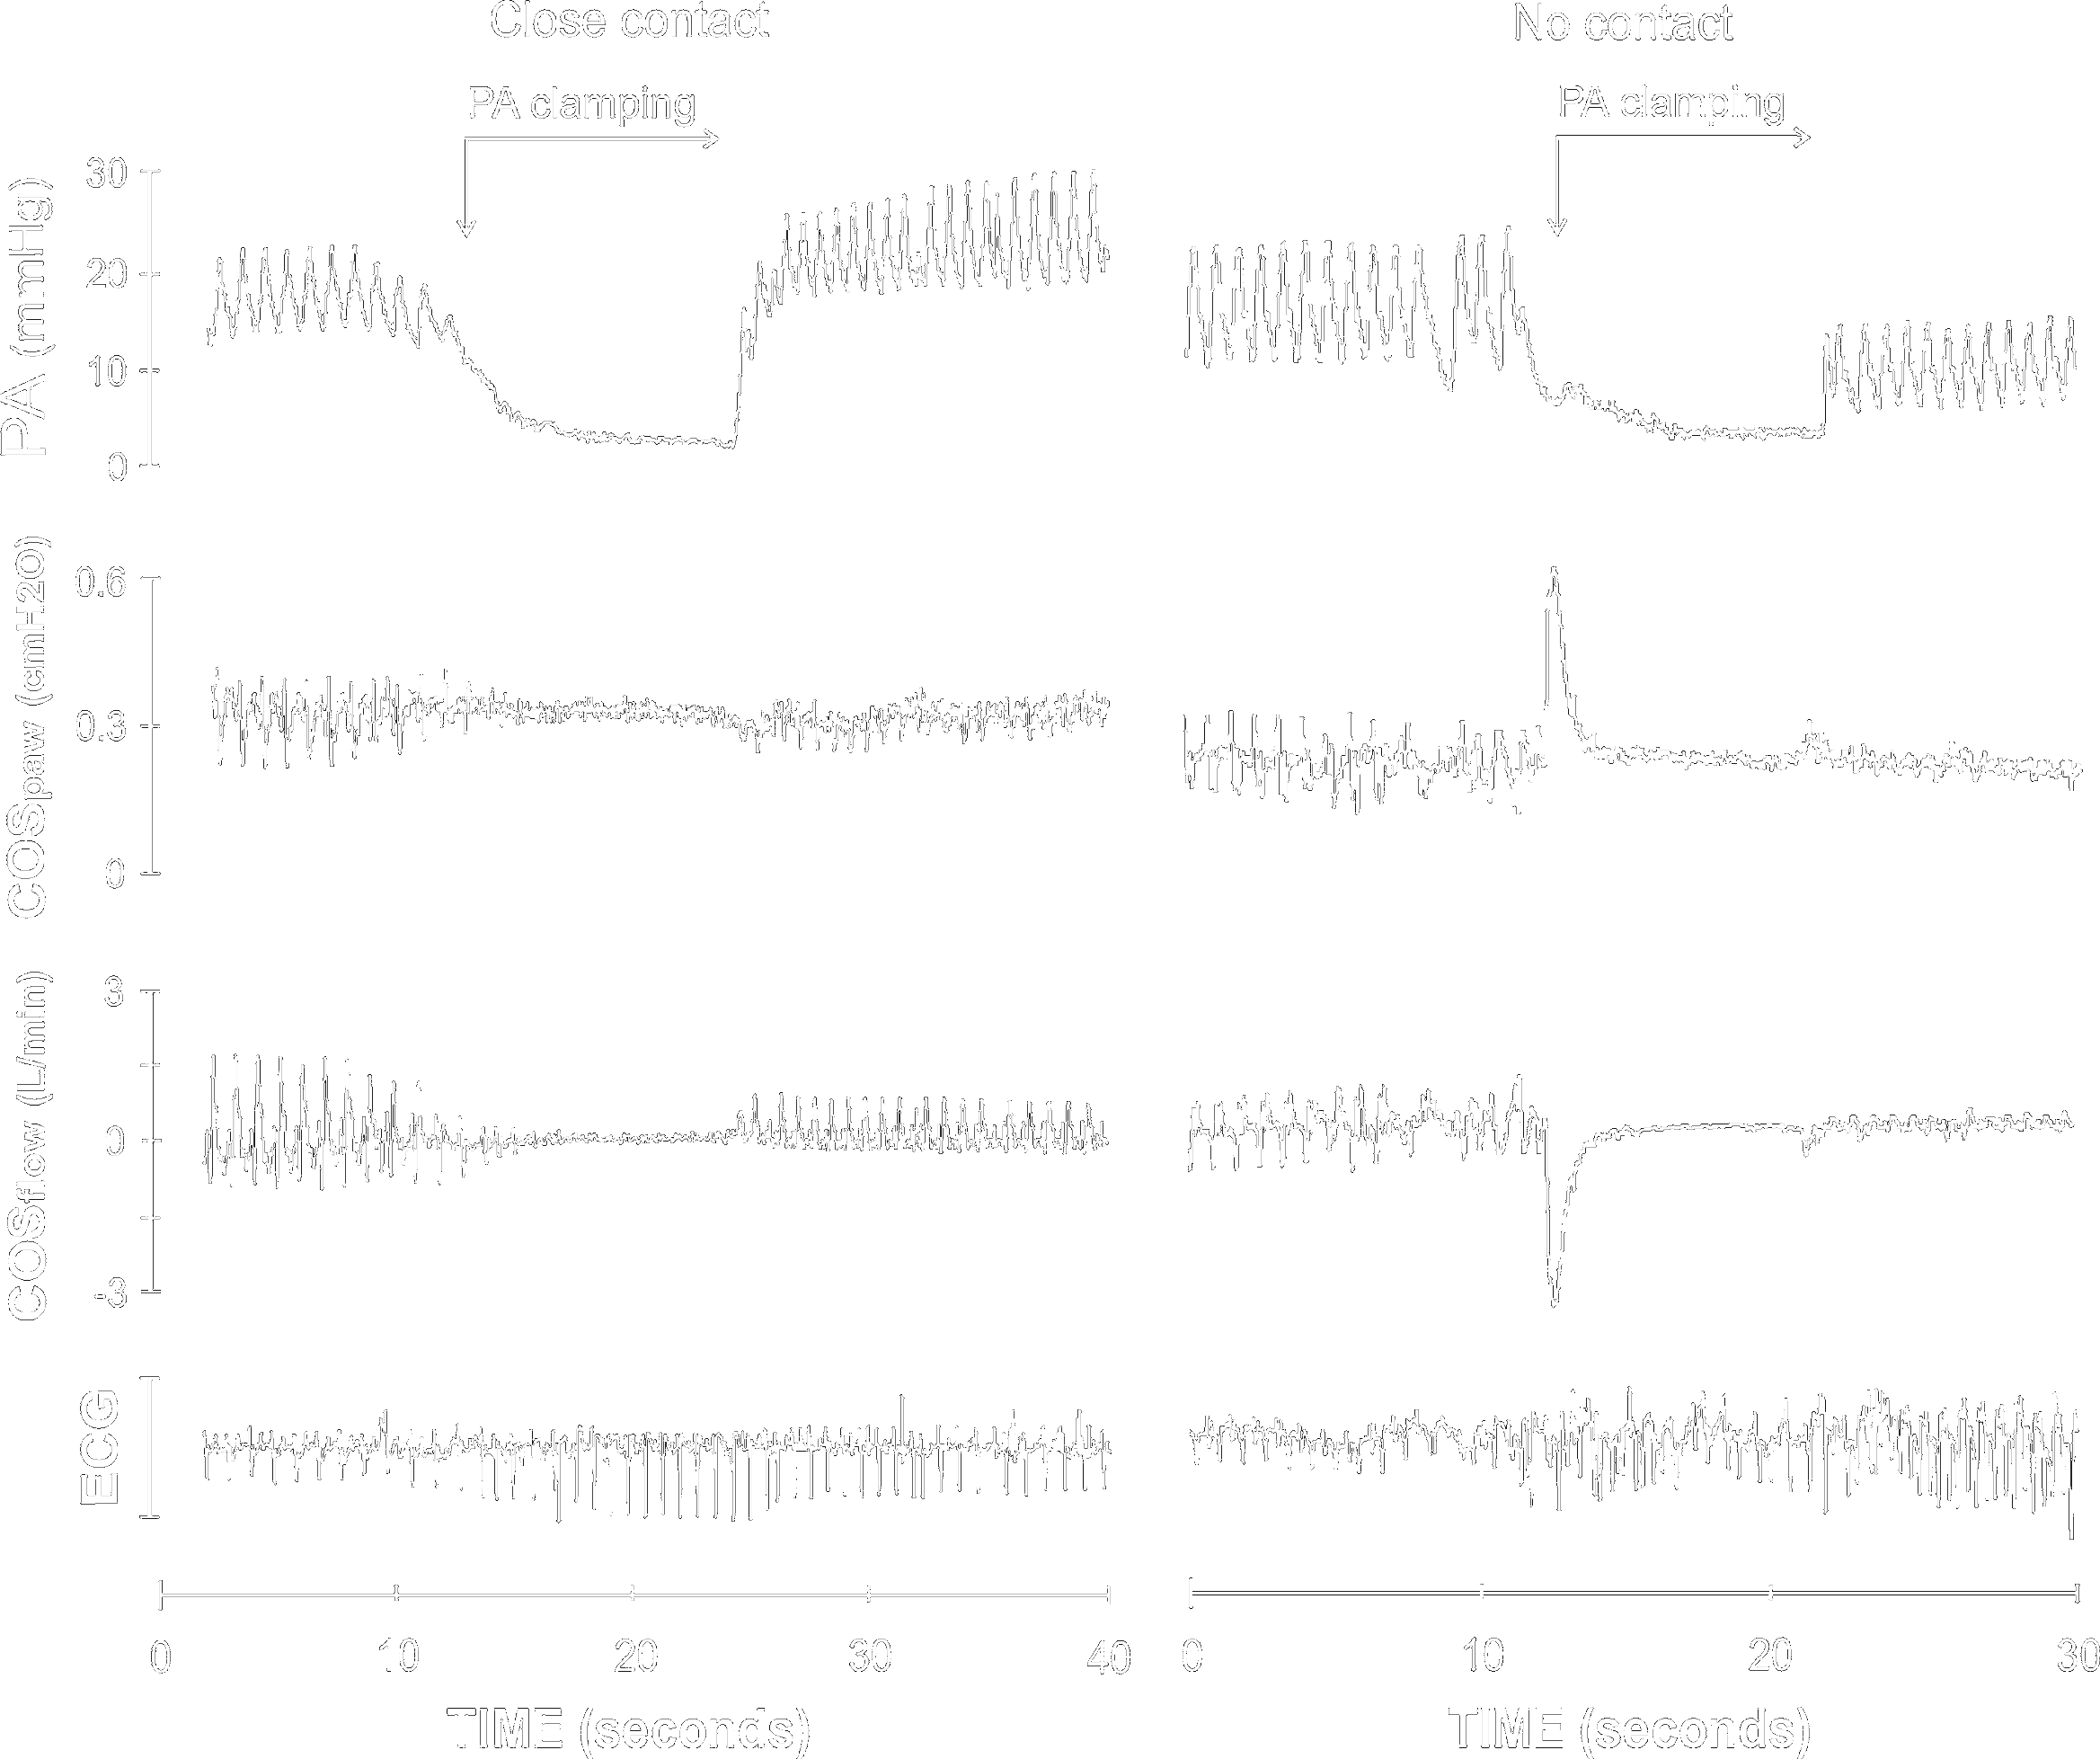
\includegraphics[height=0.85\textheight]{captures/Suarez2013-transparent}
\end{frame}
